\chapter{基本维护和安全防护}
\label{basic-maintenance}

\begin{intro}
  上一章我们认识到了「网络世界的险恶」——各种垃圾软件层出不穷、安装捆绑无处不在。
  在这样的环境之下,掌握电脑的简单维护方法显得尤为重要。阅读完这部分内容,你将找到下面这些问题的答案:
  \begin{itemize}
    \item 不小心安装了不想要的软件,怎么卸载它们?
    \item 为什么打开有些 app 时,系统总是提示「是否运行此应用对你的电脑进行更改」?
    \item 杀毒软件?安全中心?电脑管家?到底用什么?
    \item 为什么电脑天天都在「更新」?
    \item 网络上不干净的东西这么多,我要怎么才能「洁身自好」?
  \end{itemize}
\end{intro}

掌握一定的电脑维护的方法,例如软件的卸载、流氓软件的排查,以及了解一些电脑的安全维护的策略和措施是保障我们「网上冲浪」安全的重要一环。
在这一部分,我们将了解一些常用的电脑维护技巧,以及一些电脑安全方面的常识。

\section{软件的卸载}

上一章我们介绍了软件的寻找与安装,这里我们介绍软件的卸载。
软件的安装需要通过安装包来进行,而软件的卸载则是安装的逆过程,除了删除软件自身的文件之外,还会撤销一些写入系统的修改,解除一些文件关联等。
因此,软件的卸载也需要通过软件自身提供的卸载工具进行,而不是直接「删除」了事。

在 Windows 10 系统上,一般的软件卸载可以按下面的步骤进行:

\begin{itemize}
  \item 打开系统【设置】。
  \item 选择【应用】:
    \begin{figure}[htb!]
      \centering
      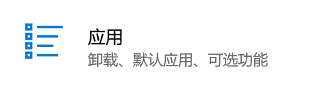
\includegraphics[width=6cm]{assets/Win_10_Apps.png}
      \caption{Windows 10 设置中的【应用】}
      \label{Win_10_Apps}
    \end{figure}
  \item 稍等片刻以使得列表完全加载。在这个界面上,会列出电脑中安装的所有软件。找到我们不想要的软件,然后点击两次【卸载】:
    \begin{figure}[thb!]
      \centering
      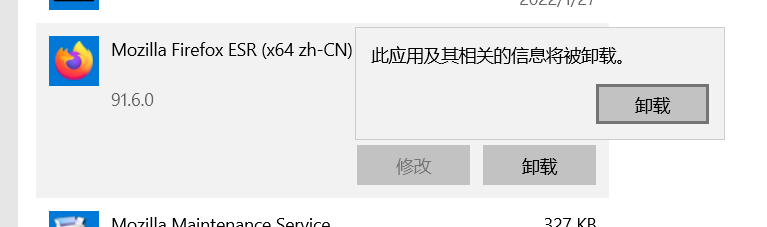
\includegraphics[width=11cm]{assets/Win_10_Uninstall.png}
      \caption{在 Windows 10 中卸载应用}
      \label{Win_10_Uninstall}
    \end{figure}
  \item 根据提示进行卸载操作即可。
\end{itemize}

而在 Windows 11 上则是这样:

\begin{itemize}
  \item 打开系统【设置】。
  \item 如图 \ref{Win_11_Apps},在界面左侧点击【应用】。
    \begin{figure}[htb!]
      \centering
      \begin{minipage}{6.5cm}
        \centering
        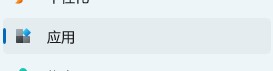
\includegraphics[width=6cm]{assets/Win_11_Apps.jpg}
        \caption{Windows 11 设置中的【应用】}
        \label{Win_11_Apps}
      \end{minipage}
      \quad
      \begin{minipage}{7cm}
        \centering
        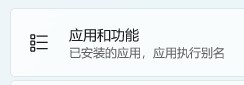
\includegraphics[width=6cm]{assets/Win_11_Apps_and_Functions.jpg}
        \caption{Windows 11 设置中的【应用和功能】}
        \label{Win_11_Apps_and_Functions}
      \end{minipage}
    \end{figure}
  \item 如图 \ref{Win_11_Apps_and_Functions},再在右侧点击【应用和功能】。
  \item 等待右侧下方的列表加载完成。这个列表就是你的电脑上安装的所有软件。找到你不想要的软件,点击这一行右侧的【\makebox[.8em]{⁝}】,再点击【卸载】:
    \begin{figure}[htb!]
      \centering
      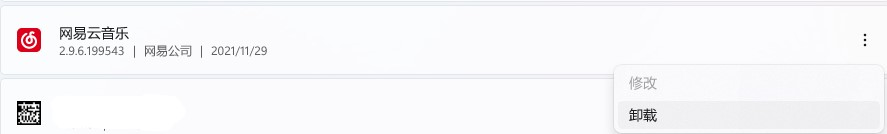
\includegraphics[width=13cm]{assets/Win_11_Unistall.jpg}
      \caption{在 Windows 11 中卸载应用}
      \label{Win_11_Unistall}
    \end{figure}
  \item 之后根据提示卸载即可。
\end{itemize}

一般来说,卸载很快就能完成。但需要特别注意的是,\regcolor{一些国产软件的卸载界面错综复杂,充斥有大量的无关选项(例如「再想想」「我要重装」等长得巨大却又不是继续卸载的按钮),因此在点选时务必十分小心。甚至有些国产软件在卸载完成后会诱导用户装一个新的其他软件,请千万注意。}
就如图 \ref{Confusing_Uninstall} 一样。

\begin{figure}[htb!]
  \centering
  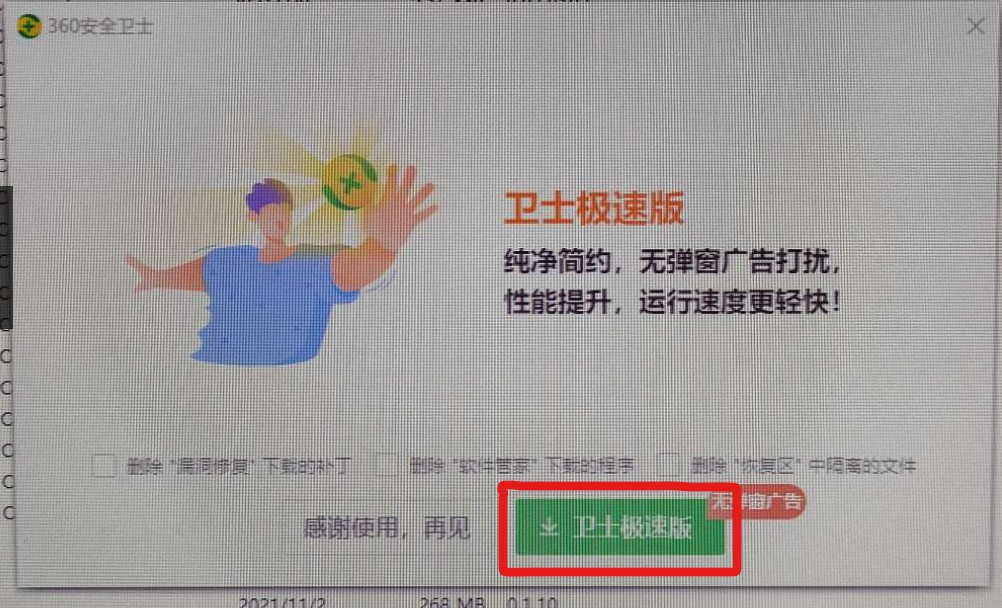
\includegraphics[width=8cm]{assets/Confusing_Uninstall.jpg}
  \caption{赤裸裸的诱导安装}
  \label{Confusing_Uninstall}
\end{figure}

卸载完成之后,可能需要重启电脑使得卸载完全进行。

\section{应用的权限与 UAC 弹窗}

这一节我们简单介绍 Windows 系统中的权限机制\footnote{如果你在使用中压根没见过如图 \ref{UAC} 一样的窗口(即 UAC 弹窗),那么这一整节的内容对你可能不适用。}。
在 Windows 系统中,一个程序(「可执行文件」,或者说 app)在一开始启动时仅被赋予了有限的「权限」——它不能更改系统的一些关键设置,不能在系统中安装新的软件,不可以动一些关键数据。
对于大多数程序来说,这有限的权限够用了:一般 app 也不会去动那些系统级的设置或者给你装一个什么新软件。
它们只需要「安分守己」地读写自己的文件,帮助用户完成工作就可以了。

但是,在一些特殊的情况下,这种有限的权限对程序来说会变得不够用。例如:

\begin{itemize}
  \item 对于\regcolor{安装包}来说,安装包本身的工作就是安装新的软件,而有限的权限禁止了这种行为。
  \item 对于一些\regcolor{专业软件}来说,它需要连接到一些系统级的部件才能工作,而有限的权限禁止了这种行为。
  \item 对于一些\regcolor{「系统优化」类的软件}来说,它本身就是需要更改系统设置的,而有限的权限禁止了这种行为。
\end{itemize}

\begin{wrapfigure}{r}{6.5cm}
  \centering
  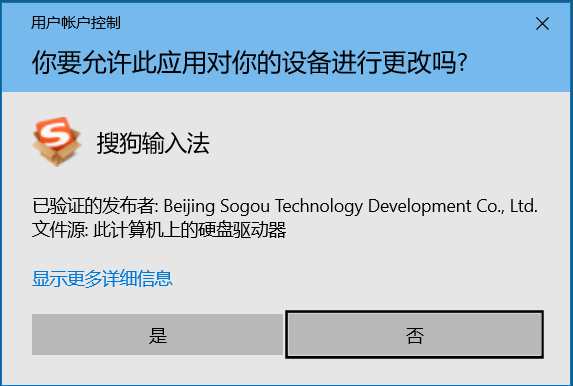
\includegraphics[width=6cm]{assets/UAC.png}
  \caption{一个 UAC 弹窗}
  \label{UAC}
\end{wrapfigure}

此时,程序需要「提升自己的权限」来完成自己的工作,这个过程称为「提权」。
而下面展示的这种弹窗(「你要允许此应用对你的设备进行更改吗」,称为「UAC 弹窗」),则是程序在向系统申请「提权」时,系统对用户的提示。
这样就能解释,为什么在大多数安装或者卸载软件的时候,系统都会弹出这个窗口询问我们;而只有我们点击【是】,安装或者卸载才能正常继续了。

那么这种「UAC 弹窗」的意义是什么呢?
想象一下这个场景:你电脑上的某个垃圾软件留下的「种子」正在蠢蠢欲动,想要给你电脑安装一套流氓软件。
然而,在一开始,这枚「种子」是没有足够权限的,因此它邪恶的计划就这样直接被粉碎了——没有提升的权限,它就没有办法进行软件安装。
这也告诉了我们一个重要的事实:\regcolor{如果电脑没有操作就弹出了不明的「UAC 弹窗」,请一律拒绝。}

一般来说,「提权」这件事是软件自行向系统申请的。
但是有一些软件设计时考虑不周全,它不会自行向系统申请「提权」,但它正常工作又必须有提升的权限。
对于这样的软件,我们可以在启动它时点击右键,选择【以管理员身份运行】,在 UAC 弹窗中选择【是】,就可以手动赋予这个软件提升的权限了。
或许你会在使用中发现,一些老旧的 app 在安装时就常常需要这么做。

当然,这一套权限系统是有很多空子的。
「提升的权限」具有从属关系——如果某个 app 得到了提权,那么由它打开的其他程序也默认具有特权。
因而,如果你为一个不怀好意的 app 赋予特权,那它就可以为所欲为了——因为它能够静默地赋予其他程序特权,然后做一些不好的事情。
因而,最终我们还是需要控制住自己电脑上软件的来源,不要让「不干净」的软件来到我们的电脑上。因此,\regcolor{不运行来源不明的可执行文件},是保证安全的根本。

\section{合理使用杀毒软件和安全软件}

合理使用杀毒软件和 / 或安全软件可以保护你的电脑安全,然而不合理地使用它们,会极大地影响我们对电脑的使用体验。
这里我们会介绍一些相对「合理」的使用这类软件的方法。

首先,\regcolor{永远不要在电脑上同时安装多于一个杀毒软件}。
例如,安装了「360 安全卫士」或者「360 杀毒」,就不要再安装「火绒安全」或者「腾讯电脑管家」。
如果你同时安装多个杀毒软件,不仅没有必要,它们之间还会因权限冲突而互相「攻击」\CJKsout*{(这就是养蛊)}。

\regcolor{警惕「全家桶」}。
以「360 安全卫士」为例,它会以各种方式提示用户安装包括但不限于「360 安全浏览器」「360 极速浏览器」「360 压缩」「鲁大师」「360 游戏大厅」「360 软件管家」等一整套 360 系的产品。
而事实上,我们只是希望安装一款安全软件或杀毒软件来保护我们的电脑罢了。
稍不留神,这些软件就会因为某个勾勾没有去掉而来到我们的电脑上。

我们安装安全软件是为了保障电脑的安全,而不是希望这些软件来拖慢我们电脑的运行速度。
然而,鉴于国产软件普遍「毒瘤」的性质,合理地使用这些软件,也需要我们对它们进行「调教」。
具体地说,我们可以\regcolor{关闭那些无用的弹窗和提示},例如每次开机时恼人的「用时 xx 秒,打败全国 xx 人」的提示,桌面上碍事的「一键加速」加速球,各种「资讯」弹窗广告和「猜你喜欢」搜索框等。
这些东西与「安全」毫不相关,反而极大影响使用体验。

随着《Missing》「软件篇」的更新,我们将会推荐一些相对优秀的杀毒软件和安全软件。

\section{Windows 更新——让人又爱又恨的「更新」}

Windows 一直在不断的更新之中——这里的「更新」指的不是诸如「Windows 7」「Windows 10」这样的大版本的更新,而是那时不时阻碍我们关机睡觉的「Windows 更新」。
打开电脑的【设置】,Windows 10 选择【更新与安全】、Windows 11 选择【Windows 更新】,你就能看到现在可用的一些 Windows 更新以及它们的状态。

\begin{figure}[htb!]
  \centering
  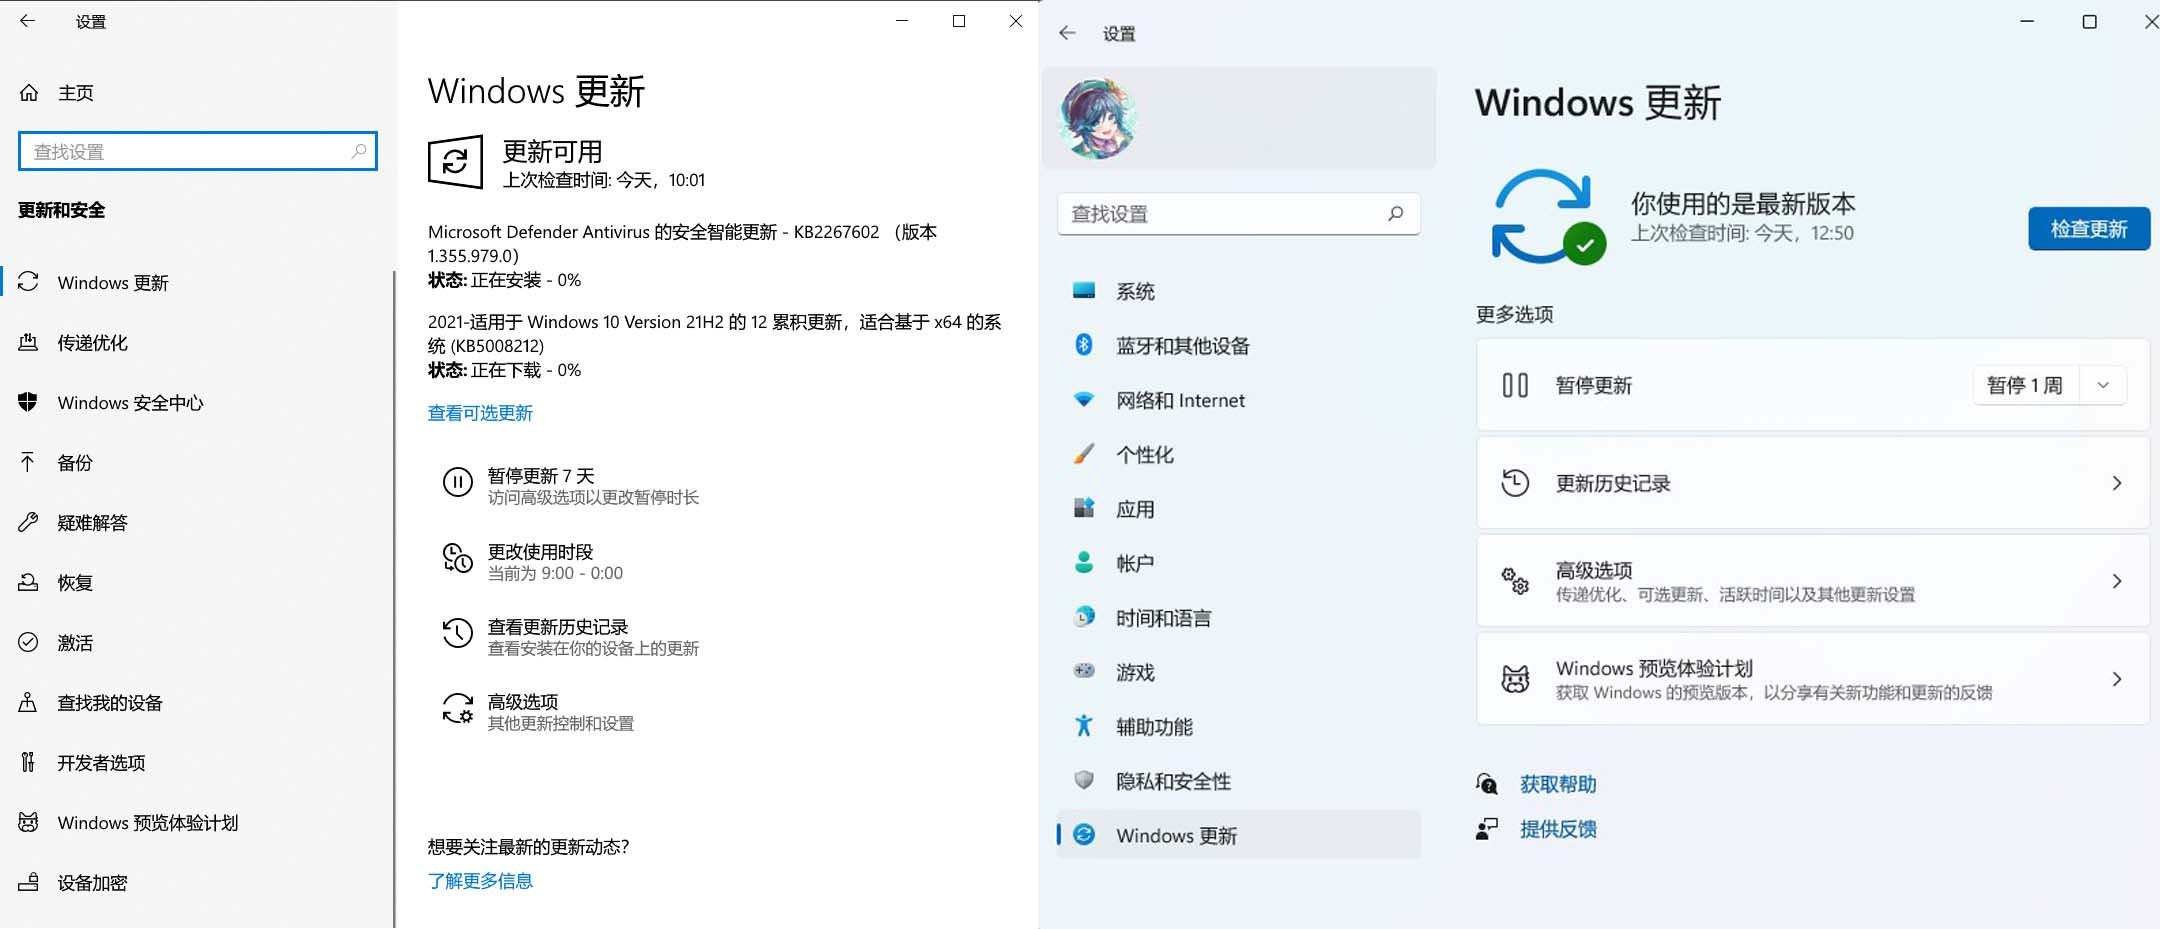
\includegraphics[width=13cm]{assets/Windows_Update.jpg}
  \caption{Windows 10 (左)与 Windows 11(右)的「Windows 更新」界面}
  \label{Windows_Update}
\end{figure}

在今天的 Windows 10 或者 Windows 11 系统中,Windows 更新主要会包括以下这些内容:

\begin{itemize}
  \item Windows 系统本身的补丁。其中包括一些对系统高危安全漏洞的「修补」,是微软给 Windows 中存在的安全问题的补丁。
  \item 电脑驱动程序的更新。这保证了你电脑上运行的驱动程序是最新的,(理论上)能更好地发挥电脑的性能。
  \item 电脑的「体验更新」。这是一些最直观的更新,主要包括系统外观与体验的优化。相比上面两项,这些更新更加容易被我们「感知」。
\end{itemize}

这样来看的话,Windows 更新应该是一件人见人爱的美事。
但事实并不是这样。
除了阻碍我们关机睡觉之外,Windows 更新是有一定风险的——那些第一晚跑 Windows 更新,然后第二早电脑就无法启动的「翻车」事件已是屡见不鲜。
事实上,Windows 更新和我们手机的「系统更新」本质一样,都会触碰系统最核心的部分。
如果这个过程中出了一些差错,就可能让系统损坏,轻则功能不正常,重则完全无法启动。

但我们不至于因噎废食,而且还是基本上噎不着的情况下。
事实上,上文所说的因为 Windows 更新导致系统损坏的情况,大都是因为用户在电脑更新时手动打断,而非 Windows 更新自身的问题。
Windows 更新提供了大量的系统安全补丁和更新,它们对保护系统安全的意义相当重大。
所以,仅仅为了可能因不当操作损坏电脑就禁用 Windows 更新并不理智,况且,现在完全关闭 Windows 更新的步骤也挺复杂。

因此,我们所需要做的,就是「正确」对待 Windows 更新。
保证 Windows 更新的安全的最重要前提,就是\regcolor{不要打断 Windows 更新}。
事实上,在系统更新的过程中,屏幕上就会一直提示你「请不要断开电源」。
在 Windows 更新进行的过程中,我们强烈建议将电脑(包括笔记本电脑,即使它内部装有电池,即使电池是充满电的)始终连接到交流电源,同时也不要盖上笔记本的盖子,为的是让系统「不受打扰」地完成整个更新流程。

\section{远离流氓软件}

所谓流氓软件,就是指会恶意诱导用户下载、安装其他软件,「传染性」强,且难以卸载的软件。
还记得在上一章中,我们亲眼目睹了由一个不干净的「高速下载器」捆绑安装的一大群软件吗?
这个「高速下载器」就是典型的流氓软件,它所安装的这些软件中有不少更是「流氓软件」。
流氓软件具有「传染性」,即一个流氓软件可能捆绑 5 个流氓软件下来,而这 5 个则可以捆绑更多其他流氓。
最后落得的,就是一台被「玩坏了」的电脑(实验过程中,并没有任何真实电脑遭受伤害):

\begin{figure}[htb!]
  \centering
  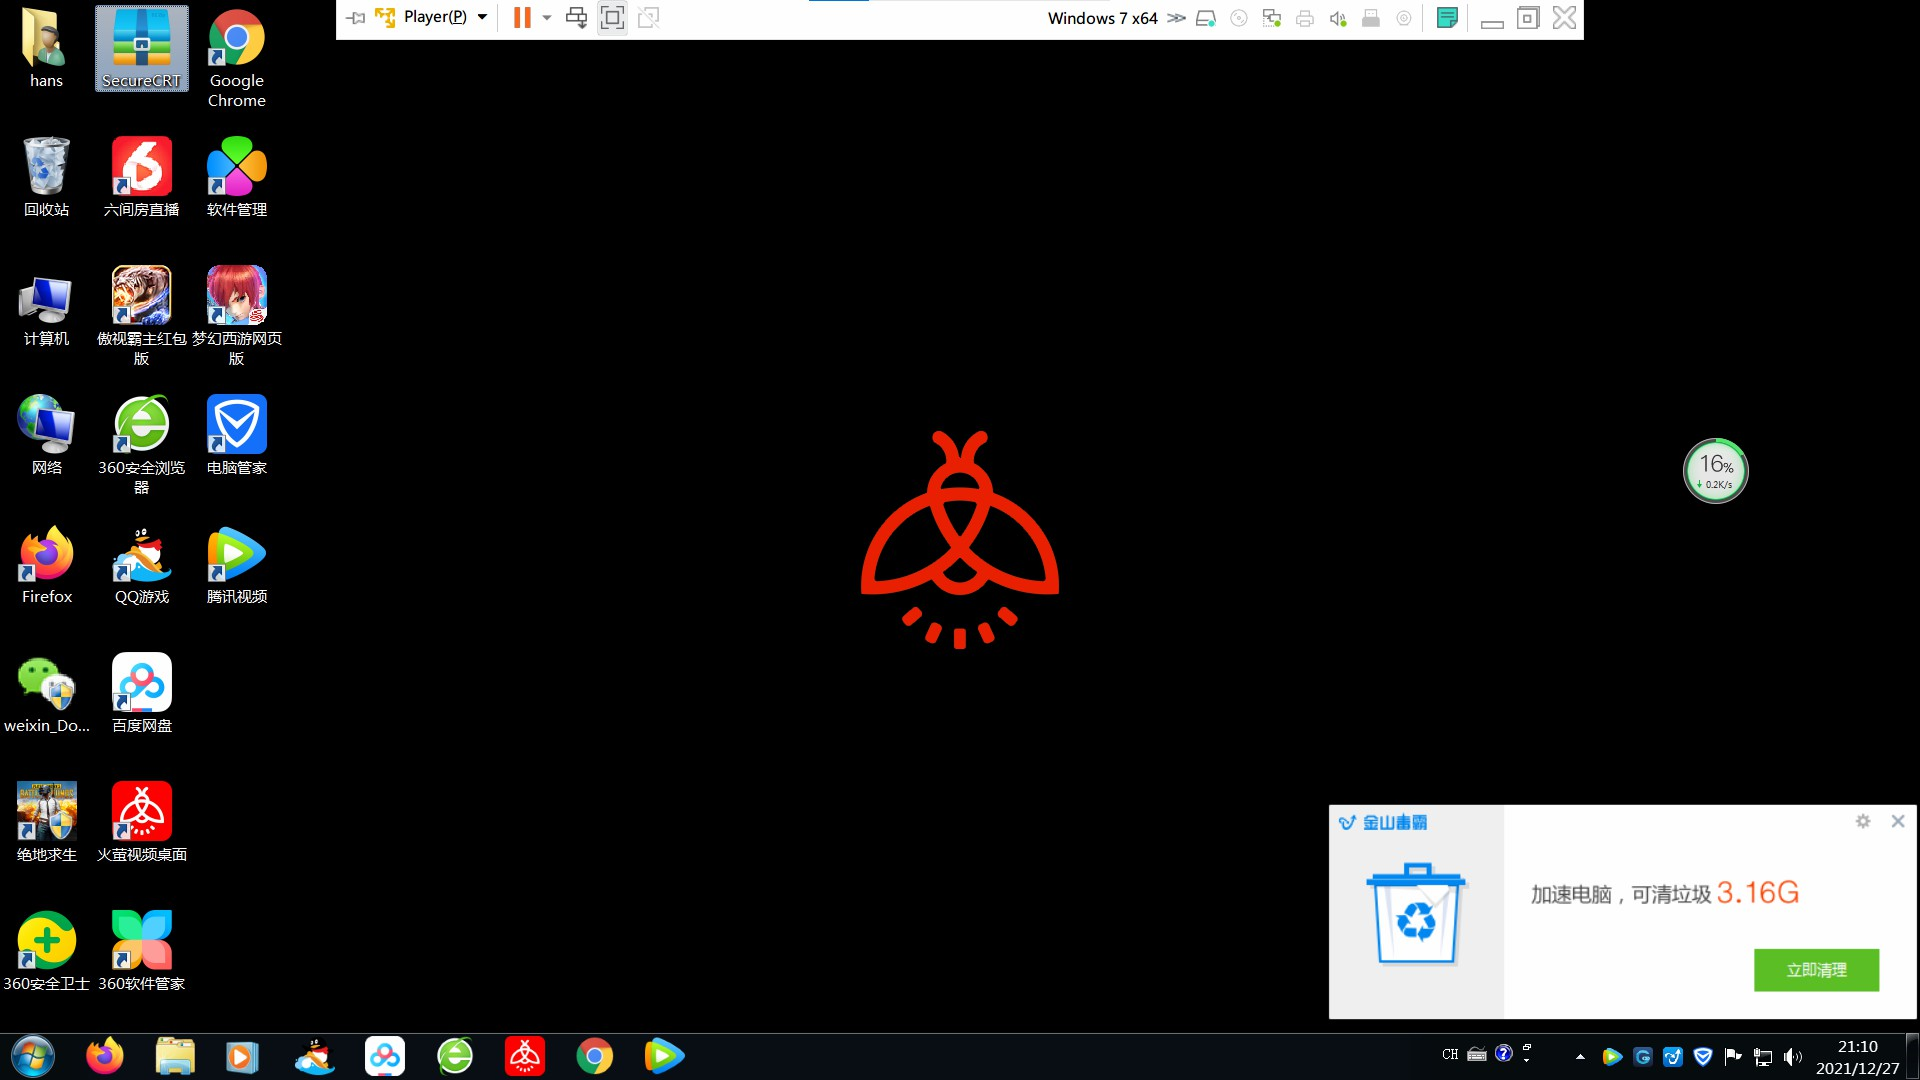
\includegraphics[width=12cm]{assets/Computer_In_A_Mess.jpg}
  \caption{被「玩坏了」的电脑}
  \label{Computer_In_A_Mess}
\end{figure}

\begin{warning}
  \centering
  远离流氓软件!\par
  \large 远离流氓软件!\par
  \LARGE 远离流氓软件!\par
\end{warning}

如果你在电脑上发现了流氓软件,请卸载它们。
一般情况下,对这些软件使用正常的卸载流程是可以完成卸载的。
但\regcolor{特别注意卸载时的捆绑勾选}。
然而有些时候,部分流氓软件会出现「卸载后卷土重来」的情况,这是因为它的安装被一个上级软件控制着,使得你的电脑在联网时会自动安装流氓软件。
此时,不妨想想最近是否为一些奇怪的软件赋予了特殊权限,然后找出上级软件,优先卸载,再去卸载其他流氓软件。

下面列出了一些\regcolor{常见的流氓软件}:

\begin{itemize}
  \item 「2345」家族,包括「2345 浏览器」「2345 好压」「2345 电脑管家」「2345 看图王」等一系列软件。
  \item 「快压」「巧压」「微压」「布丁压缩」「52 好压」等一批压缩工具。
  \item 「飞速 PDF」「小树 PDF」「熊猫 PDF」「极光 PDF」等一批 PDF 查看器。
  \item 「新速头条」等资讯类弹窗软件。
  \item 「小黑记事本」等小工具类软件。
  \item 「布丁桌面」「海螺桌面」「火萤视频桌面」等「桌面」类软件。
  \item 「手机模拟大师」「Steam 游戏助手」「傲视霸主」等游戏类软件。
\end{itemize}

清单总是有限的,但流氓软件是无穷多的。
一言以蔽之,所有非你主动安装而出现在电脑上的软件,一律认定为流氓软件。
\CJKsout*{(不会吧不会吧,不会有人自己去装流氓软件吧)}

\practice

\begin{enumerate}
  \item 在图 \ref{Q_4_1} 所示的界面中,按哪个按钮可以卸载?
  \item 在图 \ref{Q_4_2} 所示的界面中,按哪个按钮可以卸载?
  \item 在图 \ref{Q_4_3} 所示的界面中,按哪个按钮可以卸载?
  \item 在图 \ref{Q_4_4} 所示的界面中,如何操作可以卸载?
    \begin{figure}[htb!]
      \centering
      \begin{minipage}{5.5cm}
        \centering
        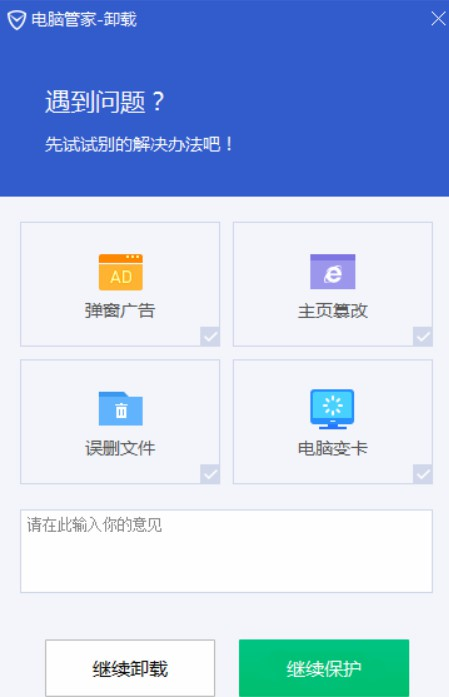
\includegraphics[width=5cm]{assets/Q_4_1.jpg}
        \caption{第1题图}
        \label{Q_4_1}
      \end{minipage}
      \qquad
      \begin{minipage}{7.5cm}
        \centering
        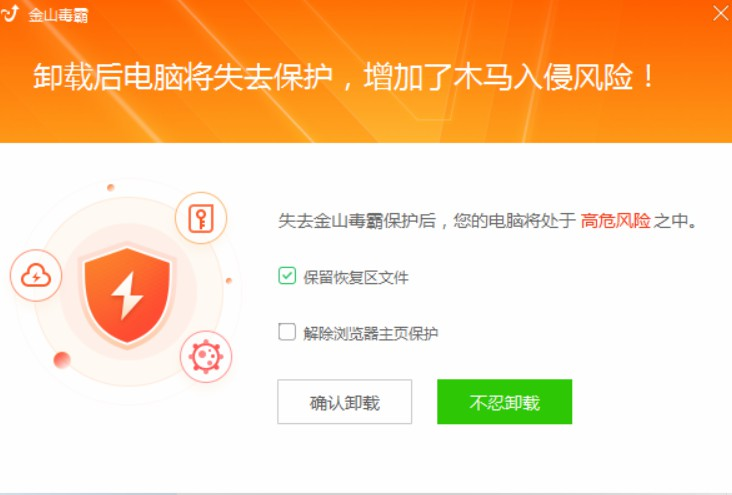
\includegraphics[width=6.8cm]{assets/Q_4_2.jpg}
        \caption{第2题图}
        \label{Q_4_2}
      \end{minipage}
      \\\vspace*{2ex}
      \begin{minipage}{6.7cm}
        \centering
        
\includegraphics[width=6.3cm]{assets/Q_4_3.jpg}
        \caption{第3题图}
        \label{Q_4_3}
      \end{minipage}
      \quad
      \begin{minipage}{6.3cm}
        \centering
        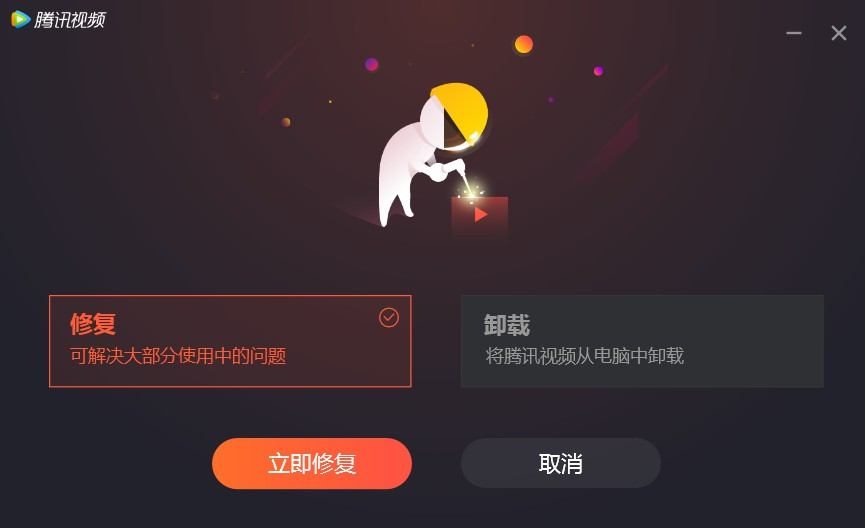
\includegraphics[width=6.2cm]{assets/Q_4_4.jpg}
        \caption{第4题图}
        \label{Q_4_4}
      \end{minipage}
    \end{figure}
  \item 清理电脑上的杀毒软件 / 安全软件,保留一个你用得最熟悉的。
    \CJKsout*{如果不知道哪个杀毒软件比较好,请看《Missing》软件篇。}
\end{enumerate}